\documentclass[10pt, a4paper]{article}
\usepackage{geometry}
\geometry{a4paper,total={6in, 8in}, margin=0.25in}
\usepackage{booktabs}
\usepackage{amssymb}
\usepackage{graphicx}
\DeclareGraphicsExtensions{.png}
\usepackage[normalem]{ulem}
\usepackage{tikz}
\usepackage{color}
\usepackage{scalerel}
\usepackage{stackengine}

\newcommand\showdiv[1]{\overline{\smash{\hstretch{.5}{)}\mkern-3.2mu\hstretch{.5}{)}}#1}}
\newcommand\ph[1]{\textcolor{white}{#1}}

\begin{document}

\begin{enumerate}
% 1
\item\mbox{}\textbf{Channel Rates and Shared Media}\\
    You are entrusted with the design of a network to interconnect a set of geographically distributed hosts within your corporation. After some research, you narrow the options to two choices, a fiber-based or a copper-based network. The pertinent statistics appear in the table below.
    \begin{center}
        \begin{tabular}{|c|c|c|}
            \hline
            Type & fiber-based network & copper-based network\\
            \hline
            signal bandwidth & 10 MHz & 1 MHz\\
            \hline
            signal-to-noise ratio at transmitter & 20 dB & 20 dB\\
            \hline
            attenuation rate & 1 dB/km & 2 dB/km\\
            \hline
        \end{tabular}
    \end{center}
    The longest link in the network in either case is 10 km.
    \begin{enumerate}
    \item What link bandwidth is possible according to Shannon's Law
        \begin{enumerate}
        \item for the fiber network?\\
            \color{blue}
            $\because$ the attenuation rate for fiber-based netork is 1 dB/km\\
            $\therefore$ the worst signal-to-noise ratio at receiver is $20 - 1 \times 10 = 10 (\mbox{dB})$\\
            $\Rightarrow 10 = 10\ log_2(SNR)$\\
            $\Rightarrow SNR = 10$\\
            $\mbox{link bandwidth} = \mbox{B}\log_2(1 + SNR) = 10 \times 10^6 \times \log_2 (1 + 10)$\\
            $\simeq 34.59 \times 10^6 (bps)$\\
            $= 34.59 (Mbps)$
            \color{black}
        \item for the copper network?\\
            \color{blue}
            $\because$ the attenuation rate for copper-based netork is 1 dB/km\\
            $\therefore$ the worst signal-to-noise ratio at receiver is $20 - 2 \times 10 = 0 (\mbox{dB})$\\
            $\Rightarrow 0 = 10\ log_2(SNR)$\\
            $\Rightarrow SNR = 1$\\
            $\mbox{link bandwidth} = \mbox{B}\log_2(1 + SNR) = 1 \times 10^6 \times \log_2 (1 + 1)$\\
            $= 1 \times 10^6 (bps)$\\
            $= 1 (Mbps)$
            \color{black}
        \end{enumerate}
    \item Assuming that hosts in the copper network can all transmit at their link rate (the values found in part (a)) simultaneously, roughly how many hosts are necessary for the networks to provide equal aggregate bandwidth (the sum of bandwidth for all hosts)?\\
        \color{blue}
        From (a),\\
        $34.59 / 1 = 34.59 \simeq 35$\\
        $\Rightarrow$ 35 hosts are necessary for the networks to provide equal aggregate bandwidth.
        \color{black}
    \item Using the copper-based network with a 32-point QAM encoding, what modulation rate (baud) is necessary to obtain the bandwidth found in part (a)?\\
        \color{blue}
        32-point QAM encoding denotes $\log_232 = 5$ bits per symbol\\
        Suppose $x$ baud is necessary to obtain the bandwidth found in part (a)\\
        $x \times 5 = 1 \times 10^6$\\
        $\Rightarrow x = 2 \times 10^5 (baud)$
        \color{black}
    \end{enumerate}
% 2
\item\mbox{} \textbf{Medium Access Control}\\
    This question concerns medium access control on a network using carrier sense multiple access with collision detection (CSMA/CD, the algorithm used with Ethernet). The network consists of four hosts distributed as shown in the figure below. The medium are broadcast, and the signal travels directly along a line of sight from sender to all receivers. Assume that the signals propagate at the speed of light in a vacuum, $3 \times 10^8 m/sec$
    \begin{center}
        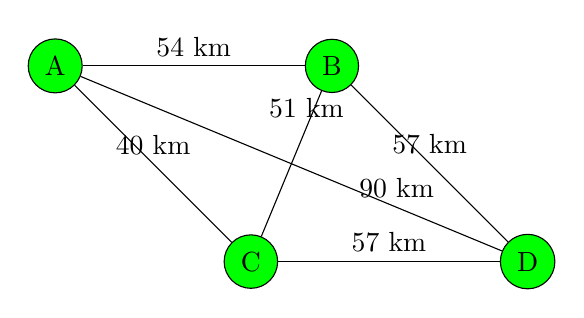
\begin{tikzpicture}
            \tikzstyle{main node}=[draw,auto,node distance=100pt,circle,align=center,fill=green]
            \node[main node] (A) {A};
            \node[main node] (B) [right of=A] {B};
            \node[main node] (C) [below right of=A] {C};
            \node[main node] (D) [below right of=B] {D};

            \draw (A) -- (B) node[draw=none,fill=none,midway,above] {54 km};
            \draw (A) -- (C) node[draw=none,fill=none,midway,above] {40 km};
            \draw (A) -- (D) node[draw=none,fill=none,near end,above] {90 km};
            \draw (B) -- (C) node[draw=none,fill=none,near start,above] {51 km};
            \draw (B) -- (D) node[draw=none,fill=none,midway,above] {57 km};
            \draw (C) -- (D) node[draw=none,fill=none,midway,above] {57 km};
        \end{tikzpicture}
    \end{center}
    \begin{enumerate}
    \item If a transmitter sends at 1 Mbps, how long must packets be to guarantee collision detection by the transmitter?\\
        \color{blue}
        The longest path in the network $= 90 (km) = 90 \times 10^3 (m)$\\
        Round trip time of the longest path $= 2 \times \frac{90 \times 10^3}{3 \times 10^8} = 600 \times 10^{-6} (s) = 600 (\mu s)$\\
        Minimum packet size to guarantee collision detection by the transmitter $= 600 \times 10^{-6} \times 1 \times 10^6 = 600 (bit) = 75 (B)$
        \color{black}
    \item Divide time into slots the length of the maximum round-trip propagation delay in the network. One packet may be transmitted each time slot. Assume that each of the four hosts attempts to transmit with probability $p$ in each time slot. What is the probability of a successful transmission in any given slot if
        \begin{enumerate}
        \item $p = \frac{1}{4}$\\
            \color{blue}
            $C_1^{4} \times p \times (1 - p)^3 = C_1^{4} \times \frac{1}{4} \times (1 - \frac{1}{4})^3 = \frac{27}{64}$
            \color{black}
        \item $p = \frac{1}{2}$\\
            \color{blue}
            $C_1^{4} \times p \times (1 - p)^3 = C_1^{4} \times \frac{1}{2} \times (1 - \frac{1}{2})^3 = \frac{1}{4}$
            \color{black}
        \item $p = \frac{3}{4}$\\
            \color{blue}
            $C_1^{4} \times p \times (1 - p)^3 = C_1^{4} \times \frac{3}{4} \times (1 - \frac{3}{4})^3 = \frac{3}{64}$
            \color{black}
        \end{enumerate}
    \item Using the minimum transmission length from part (a) and the probability of successful transmission from part (b)(ii) (for $p = \frac{1}{2}$), calculate the average throughput of the network if each packet requires 20 bytes of header/trailer and
        \begin{enumerate}
        \item 10 bytes of data, and\\
            \color{blue}
            From (a), the packet size is $75 (B)$. From (b)(ii), the probability of successful transmission is $\frac{1}{4}$\\
            The minimum packet size is 75B. Therefore, if the sum of the header/trailer and data is less than 75B, padding bytes must be added.\\
            $\Rightarrow$ the average throughput of the network is $\frac{1}{4} \times \frac{10}{75} \times 1 \times 10^6 \simeq 33.3 \times 10^3 (bps)$\\
            $= 33.3 (Kbps)$
            \color{black}
        \item 50 bytes of data.\\
            \color{blue}
            From (a), the packet size is $75 (B)$. From (b)(ii), the probability of successful transmission is $\frac{1}{4}$\\
            The minimum packet size is 75B. Therefore, if the sum of the header/trailer and data is less than 75B, padding bytes must be added.\\
            $\Rightarrow$ the average throughput of the network is $\frac{1}{4} \times \frac{50}{75} \times 1 \times 10^6 \simeq 166.7 \times 10^3 (bps)$\\
            $= 166.7 (Kbps)$
            \color{black}
        \end{enumerate}
    \end{enumerate}
% 3
\item\mbox{}\textbf{Workstations as Switches}\\
    You are entrusted with the purchase of a workstation to serve as a switch between two high-speed local area networks (LAN's). One of the networks is an UltraNet, a 1 Gbps LAN with 80 bytes of total overhead (headers and trailers) required for each frame. The other network is an OmniNet, a 1.3 Gbps LAN with 100 bytes of overhead required for each frame. All packets sent on either network have exactly 1,000 bytes of data. After some research, you narrow the options to the two architectures described in the table below.
    \begin{center}
        \begin{tabular}{|c|c|c|}
            \hline
            Name & Admiral J9000 & SPQ\\
            \hline
            CPU handles & 100,000 packets/second & 60,000 packets/second\\
            \hline
            Number of I/O buses & 3 & 1\\
            \hline
            I/O bus bandwidth & 480 Mbps & 1 Gbps\\
            \hline
            Memory bus bandwidth & 2 Gbps & 1.4 Gbps\\
            \hline
            Price & \$10,000 & \$8,000\\
            \hline
        \end{tabular}
    \end{center}
    \begin{enumerate}
    \item Pick one. Justify your decision, showing all work.\\
        \color{blue}
        Determine either CPU, I/O bus bandwidth, or memory bus bandwidth will be the bottleneck of the workstation:
        \begin{tabular}{lll}
            \toprule
            Name & Admiral J9000 & SPQ\\
            \hline
            CPU & $100000 \times 1000 \times 8 = 800 \times 10^6 (bps)$ & $60000 \times 1000 \times 8 = 480 \times 10^6 (bps)$\\
                & $= 800 (Mbps)$ & $= 480 (Mbps)$\\
            I/O bus bandwidth & $\frac{2 \times 480}{2} = 480 (Mbps)$ & $\frac{1}{2} = 0.5 (Gbps) = 500 (Mbps)$\\
            memory bus bandwidth & $\frac{2}{2} = 1 (Gbps)$ & $\frac{1.4}{2} = 0.7 (Gbps) = 700 (Mbps)$\\
            \bottomrule
        \end{tabular}\\

        $\because$ both Admiral J9000 and SPQ have the same bottleneck, which is $480 (Mbps)$\\
        $\therefore$ I will choose SPQ because it is cheaper
        \color{black}
    \item Draw a block diagram of the workstation architecture that you have chosen in part (a), labeling all components with appropriate names and data rates.\\
        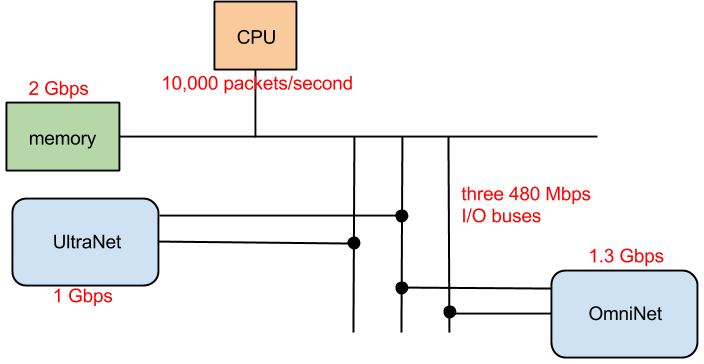
\includegraphics[width=4in]{images/p3b_block_diagram}
    \item At the maximum sustainable bandwidth (i.e., with no packets dropped), what is the transmission rate - the total number of bits per second, including headers and trailers - sent over each network link?\\
        \color{blue}
        For UltraNet, transmission rate $= 480 \times \frac{1000 + 80}{1000} = 518.4 (Mbps)$\\
        For OmniNet, transmission rate $= 480 \times \frac{1000 + 100}{1000} = 528 (Mbps)$
        \color{black}
    \end{enumerate}
% 4
\item\mbox{}\textbf{Forwarding Tables}\\
    Consider the network shown in the figure below. The links are labeled with relative costs. The three parts of this problem deal with datagram forwarding, circuit-switched forwarding, and source-routed forwarding, respectively
    \begin{center}
        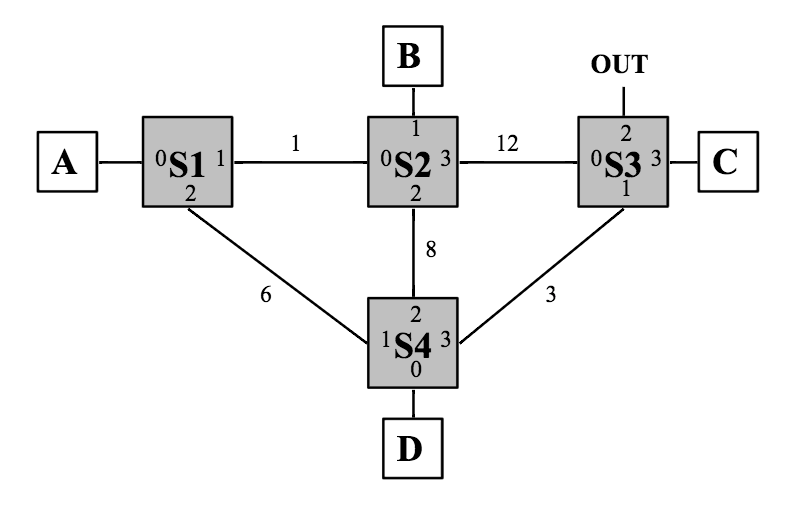
\includegraphics[width=3.5in]{images/p4_network}
    \end{center}
    \begin{enumerate}
    \item Give the datagram routing table at switch S2, assuming least-cost paths are used. Your table should consist of one row for each possible destination (including the default destination, OUT) consisting of the destination ID, output port, and distance\\
        \color{blue}
        \begin{tabular}{ccc}
            \toprule
            destination ID & output port & distance\\
            \hline
            OUT & 0 & -\\
            A & 0 & 1\\
            B & 1 & 0\\
            C & 0 & 10\\
            D & 0 & 7\\
            \bottomrule
        \end{tabular}
        \color{black}
    \item Suppose virtual circuit forwarding is used for the network shown above with the routing tables show below.
        \begin{center}
            \begin{tabular}{|c|c|c|c|c|}
                \hline
                S1: & $\mbox{port}_{\mbox{in}}$ & $\mbox{VCI}_{\mbox{in}}$ & $\mbox{port}_{\mbox{out}}$ & $\mbox{VCI}_{\mbox{out}}$\\
                \cline {2-5}
                & 0 & 0 & 2 & 0\\
                \cline {2-5}
                & 0 & 1 & 1 & 0\\
                \cline {2-5}
                & 2 & 0 & 1 & 1\\
                \hline
            \end{tabular}\qquad
            \begin{tabular}{|c|c|c|c|c|}
                \hline
                S3: & $\mbox{port}_{\mbox{in}}$ & $\mbox{VCI}_{\mbox{in}}$ & $\mbox{port}_{\mbox{out}}$ & $\mbox{VCI}_{\mbox{out}}$\\
                \cline {2-5}
                & 0 & 0 & 3 & 0\\
                \cline {2-5}
                & 0 & 1 & 2 & 1\\
                \cline {2-5}
                & 3 & 0 & 0 & 0\\
                \hline
            \end{tabular}\\

            \begin{tabular}{|c|c|c|c|c|}
                \hline
                S2: & $\mbox{port}_{\mbox{in}}$ & $\mbox{VCI}_{\mbox{in}}$ & $\mbox{port}_{\mbox{out}}$ & $\mbox{VCI}_{\mbox{out}}$\\
                \cline {2-5}
                & 0 & 0 & 2 & 0\\
                \cline {2-5}
                & 0 & 1 & 3 & 1\\
                \cline {2-5}
                & 2 & 0 & 3 & 0\\
                \cline {2-5}
                & 2 & 2 & 1 & 0\\
                \cline {2-5}
                & 3 & 0 & 1 & 1\\
                \hline
            \end{tabular}\qquad
            \begin{tabular}{|c|c|c|c|c|}
                \hline
                S4: & $\mbox{port}_{\mbox{in}}$ & $\mbox{VCI}_{\mbox{in}}$ & $\mbox{port}_{\mbox{out}}$ & $\mbox{VCI}_{\mbox{out}}$\\
                \cline {2-5}
                & 0 & 0 & 2 & 0\\
                \cline {2-5}
                & 0 & 2 & 1 & 0\\
                \cline {2-5}
                & 1 & 0 & 2 & 2\\
                \cline {2-5}
                & 2 & 0 & 0 & 0\\
                \hline
            \end{tabular}
        \end{center}
        When setting up a new virtual circuit on a given output port, a switch should assign the smallest unused virtual circuit identifier for that port. Indicate how the routing tables change after the following two (cumulative) events:
        \begin{enumerate}
        \item The circuit beginning with (port, VCI)=(0,0) at switch S1 is torn down, and\\
            \color{blue}
            \begin{tabular}{|c|c|c|c|c|}
                \hline
                S1: & $\mbox{port}_{\mbox{in}}$ & $\mbox{VCI}_{\mbox{in}}$ & $\mbox{port}_{\mbox{out}}$ & $\mbox{VCI}_{\mbox{out}}$\\
                \cline {2-5}
                & \textcolor{red}{-} & \textcolor{red}{-} & \textcolor{red}{-} & \textcolor{red}{-}\\
                \cline {2-5}
                & 0 & 1 & 1 & 0\\
                \cline {2-5}
                & 2 & 0 & 1 & 1\\
                \hline
            \end{tabular}\qquad
            \begin{tabular}{|c|c|c|c|c|}
                \hline
                S3: & $\mbox{port}_{\mbox{in}}$ & $\mbox{VCI}_{\mbox{in}}$ & $\mbox{port}_{\mbox{out}}$ & $\mbox{VCI}_{\mbox{out}}$\\
                \cline {2-5}
                & 0 & 0 & 3 & 0\\
                \cline {2-5}
                & 0 & 1 & 2 & 1\\
                \cline {2-5}
                & 3 & 0 & 0 & 0\\
                \hline
            \end{tabular}\\

            \begin{tabular}{|c|c|c|c|c|}
                \hline
                S2: & $\mbox{port}_{\mbox{in}}$ & $\mbox{VCI}_{\mbox{in}}$ & $\mbox{port}_{\mbox{out}}$ & $\mbox{VCI}_{\mbox{out}}$\\
                \cline {2-5}
                & 0 & 0 & 2 & 0\\
                \cline {2-5}
                & 0 & 1 & 3 & 1\\
                \cline {2-5}
                & 2 & 0 & 3 & 0\\
                \cline {2-5}
                & \textcolor{red}{-} & \textcolor{red}{-} & \textcolor{red}{-} & \textcolor{red}{-}\\
                \cline {2-5}
                & 3 & 0 & 1 & 1\\
                \hline
            \end{tabular}\qquad
            \begin{tabular}{|c|c|c|c|c|}
                \hline
                S4: & $\mbox{port}_{\mbox{in}}$ & $\mbox{VCI}_{\mbox{in}}$ & $\mbox{port}_{\mbox{out}}$ & $\mbox{VCI}_{\mbox{out}}$\\
                \cline {2-5}
                & 0 & 0 & 2 & 0\\
                \cline {2-5}
                & 0 & 2 & 1 & 0\\
                \cline {2-5}
                & \textcolor{red}{-} & \textcolor{red}{-} & \textcolor{red}{-} & \textcolor{red}{-}\\
                \cline {2-5}
                & 2 & 0 & 0 & 0\\
                \hline
            \end{tabular}\\
            \color{black}
        \item subsequently, a new circuit is set up from host D to host B using a least-cost path.\\
            \color{blue}
            \begin{tabular}{|c|c|c|c|c|}
                \hline
                S1: & $\mbox{port}_{\mbox{in}}$ & $\mbox{VCI}_{\mbox{in}}$ & $\mbox{port}_{\mbox{out}}$ & $\mbox{VCI}_{\mbox{out}}$\\
                \cline {2-5}
                & 0 & 1 & 1 & 0\\
                \cline {2-5}
                & 2 & 0 & 1 & 1\\
                \cline {2-5}
                & \textcolor{red}{2} & \textcolor{red}{1} & \textcolor{red}{1} & \textcolor{red}{2}\\
                \hline
            \end{tabular}\qquad
            \begin{tabular}{|c|c|c|c|c|}
                \hline
                S3: & $\mbox{port}_{\mbox{in}}$ & $\mbox{VCI}_{\mbox{in}}$ & $\mbox{port}_{\mbox{out}}$ & $\mbox{VCI}_{\mbox{out}}$\\
                \cline {2-5}
                & 0 & 0 & 3 & 0\\
                \cline {2-5}
                & 0 & 1 & 2 & 1\\
                \cline {2-5}
                & 3 & 0 & 0 & 0\\
                \hline
            \end{tabular}\\

            \begin{tabular}{|c|c|c|c|c|}
                \hline
                S2: & $\mbox{port}_{\mbox{in}}$ & $\mbox{VCI}_{\mbox{in}}$ & $\mbox{port}_{\mbox{out}}$ & $\mbox{VCI}_{\mbox{out}}$\\
                \cline {2-5}
                & 0 & 0 & 2 & 0\\
                \cline {2-5}
                & 0 & 1 & 3 & 1\\
                \cline {2-5}
                & 2 & 0 & 3 & 0\\
                \cline {2-5}
                & 3 & 0 & 1 & 1\\
                \cline {2-5}
                & \textcolor{red}{0} & \textcolor{red}{2} & \textcolor{red}{1} & \textcolor{red}{0}\\
                \hline
            \end{tabular}\qquad
            \begin{tabular}{|c|c|c|c|c|}
                \hline
                S4: & $\mbox{port}_{\mbox{in}}$ & $\mbox{VCI}_{\mbox{in}}$ & $\mbox{port}_{\mbox{out}}$ & $\mbox{VCI}_{\mbox{out}}$\\
                \cline {2-5}
                & 0 & 0 & 2 & 0\\
                \cline {2-5}
                & 0 & 2 & 1 & 0\\
                \cline {2-5}
                & 2 & 0 & 0 & 0\\
                \cline {2-5}
                & \textcolor{red}{0} & \textcolor{red}{1} & \textcolor{red}{1} & \textcolor{red}{1}\\
                \hline
            \end{tabular}\\
            \color{black}
        \end{enumerate}
    \item Now assume the use of source routing for the network. Indicate the sequence of absolute port identifier to be found in a packet header for a packet sent by host B destined for host C along the least-cost path. (Assume that the sequence of port identifier in the header is transmitted in the order written, from left to right.)\\
        \color{blue}
        0, 2, 3, 3
        \color{black}
    \end{enumerate}
% 5
\item\mbox{}\textbf{Error Detection with Cyclic Redundancy Checks}\\
    Use the CRC-8 generator polynomial $x^8 + x^2 + x + 1$ for both parts of this problem.
    \begin{enumerate}
    \item Calculate the CRC value of the bit sequence \textbf{0011\ 1100\ 0011}.\\
        \color{blue}
        $\mbox{M} = 001111000011$\\
        $\mbox{C} = 100000111, k = 8$\\
        $\mbox{T} = 00111100001100000000$\\

        \stackMath\def\stackalignment{r}
        \stackunder{100000111 \stackon[1pt]{\showdiv{00111100001100000000}}{}}{
            \Shortstack[l]{
                {\underline{100000111}}
                \ph{1}111001101
                {\ph{1}\underline{100000111}}
                \ph{12}110010100
                {\ph{12}\underline{100000111}}
                \ph{123}100100110
                {\ph{123}\underline{100000111}}
                \ph{123456}100001000
                {\ph{123456}\underline{100000111}}
                \ph{12345678901}1111000
            }
        }\\
        $\Rightarrow \mbox{CRC} = 1111000$
        \color{black}
    \item Recall that error detection with a CRC works by appending a CRC value to the message to make it a multiple of the generator polynomial. Find a 12-bit burst error polynomial $E(x) = x^{11} + ... + 1$ that cannot be detected by a CRC check (with CRC-8).\\
        \color{blue}
        We can find a 12-bit burst error polynomial $E(x)$ that cannot be detected by a CRC check if $E(x)$ is divisible by $C(x)$\\
        $\Rightarrow E(x) = (x^8 + x^2 + x + 1) \times x^3$\\
        $= x^{11} + x^5 + x^4 + x^3$
        \color{black}
    \end{enumerate}
% 6
\item\mbox{}\textbf{Spanning Tree Algorithm for Intelligent Bridges}\\
    Suppose the Perlman spanning tree algorithm and the bridge learning algorithm for forwarding are used for the network shown below.
    \begin{center}
        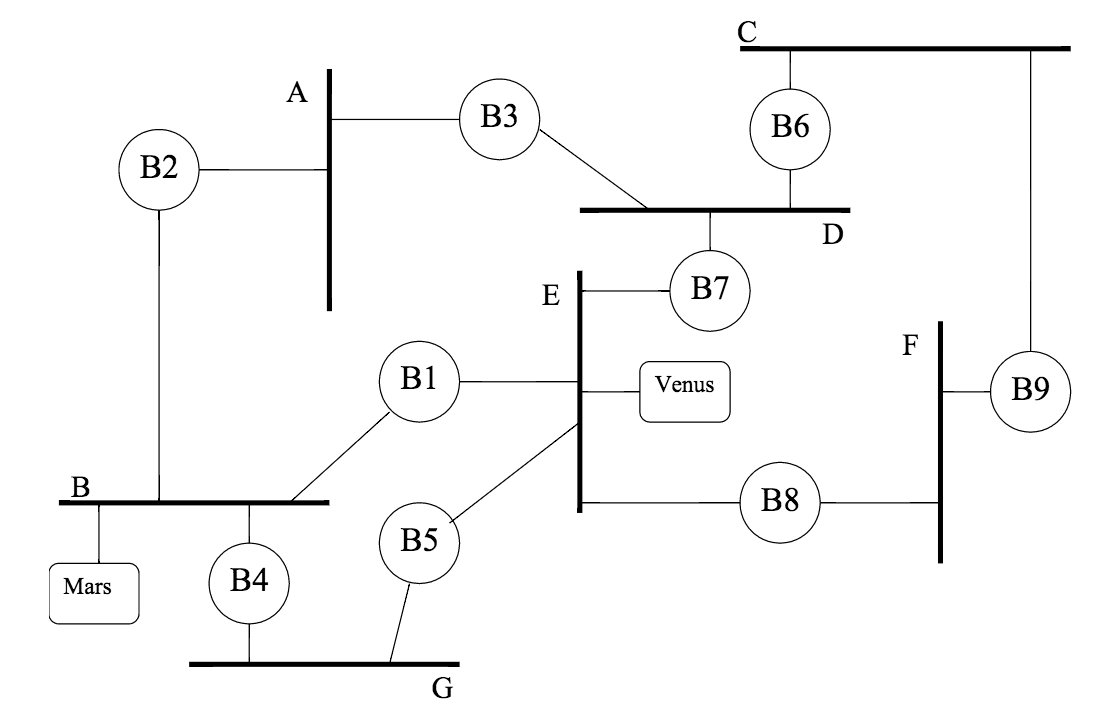
\includegraphics[width=4in]{images/p6_spanning_tree}
    \end{center}
    \begin{enumerate}
        \item Indicate which bridge is root, which ports are root ports (i.e. the preferred port for reaching the root bridge), which bridge is the designated bridge for each LAN, and which ports are designated ports (i.e. the ports that connect some LAN to its given designated bridge). Hint: bridges that are not designated bridges for any LAN, and ports that are not either root ports or designated ports do not play a role in the routing of packets. The reamaining bridges together with the LANs form a spanning tree.\\
            \color{blue}
            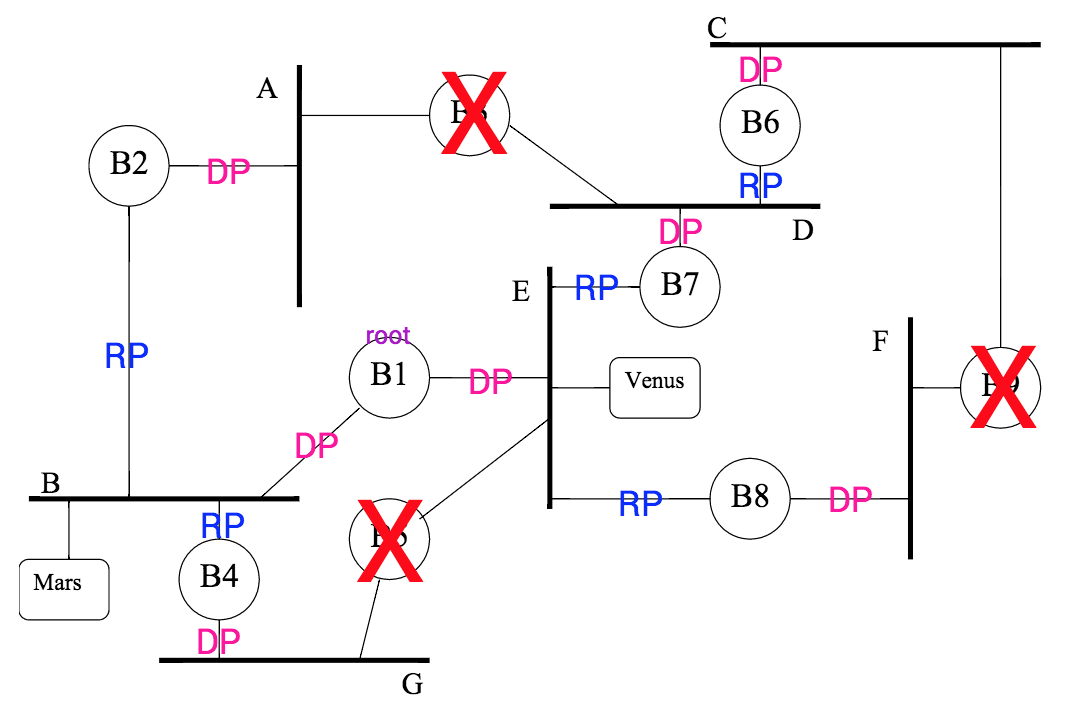
\includegraphics[width=4in]{images/p6a_spanning_tree_result}\\
            As the figure shows. B1 is the root bridge. ``RP'' denotes root port, and ``DP'' denotes designated port. Bridge B3, B5, and B9 and the ports connected to them do not from the spanning tree.\\
            The designated bridge for each LAN:\\
            \begin{tabular}{cc}
                \toprule
                LAN & designated bridge\\
                \hline
                A & B2\\
                B & B1\\
                C & B6\\
                D & B7\\
                E & B1\\
                F & B8\\
                G & B4\\
                \bottomrule
            \end{tabular}
            \color{black}
        \item Suppose after the configuration is complete, host Mars attaches to LAN B and host Venus attaches to LAN E. Suppose Mars sends a message to Venus, then Venus sends a message to Mars, then Mars sends a second message to Venus. For each of the three messages, indicate which LANs the message is heard on.
            \color{blue}
            \begin{itemize}
            \item Mars sends a message to Venus:\\
                $\because$ no bridge has learned any host's location before\\
                $\therefore$ the message will be passed by all bridges, and the message can be heard on all LANs\\
                $\Rightarrow$ ABCDEFG
            \item Venus sends a message to Mars:\\
                $\because$ all bridges have learned the location of Mars\\
                $\therefore$ bridge B2, B4, B7, and B8 will not pass the message\\
                $\Rightarrow$ EB
            \item Mars sends a second message to Venus:\\
                $\because$ bridges B1, B2, B4, B7, and B8 have learned the location of Venus\\
                $\therefore$ bridge B2, B4, B7, and B8 will not pass the message\\
                $\Rightarrow$ BE
            \end{itemize}
            \color{black}
    \end{enumerate}
% 7
\item\mbox{}\textbf{Bit- and Byte-Stuffing}\\
    Consider a data stream of 8-bit ASCII characters with values 0 to 127. Assume that the probability of a byte assuming each possible is equal (i.e., is exactly 1/128).
    \begin{enumerate}
    \item Using the bit-stuffing protocol discussed in class, what is the average number of bits that must be stuffed (inserted) per byte in the stream?\\
        \color{blue}
        $\because$ the value only ranges from 0 to 127\\
        $\therefore$ the first bit in any byte must be 0\\
        $\Rightarrow$ the possible sequences need to be stuffed:\\
        \begin{tabular}{cccccccc}
            0 & \underline{\ } & \underline{\ } & 1 & 1 & 1 & \underline{\ } & \underline{\ }\\
              & 0 & 0 & & & & 1 & 1\\
              & 0 & 1 & & & & 1 & 0\\
              & 0 & 1 & & & & 1 & 1\\
              & 1 & 0 & & & & 1 & 1\\
              & 1 & 1 & & & & 0 & 0\\
              & 1 & 1 & & & & 0 & 1\\
              & 1 & 1 & & & & 1 & 0\\
              & 1 & 1 & & & & 1 & 1\\
        \end{tabular}\\
        there are 8 possible sequences need to be stuffed\\
        $\Rightarrow$ the average number of bits that must be stuffed per byte in the stream $= \frac{8}{128} \times 1$\\
        $= \frac{1}{16}$
        \color{black}
    \item Answer the same question posed in part (a) for a byte-stuffing protocol in which the DLE character (value 16) must be escaped by stuffing a second DLE byte.\\
        \color{blue}
        the DLE character (value 16) denotes the sequence of 00010000\\
        $\Rightarrow$ the average number of bits that must be stuffed per byte in the stream $= \frac{1}{128} \times 8$\\
        $= \frac{1}{16}$
        \color{black}
    \end{enumerate}
    Now assume that the data stream contains only value in the range 32 to 127, again with a uniform probability distribution amongst the possible values.
    \begin{enumerate}
    \item Recalcuate your answer to part (a) with the new probability distribution.\\
        \color{blue}
        $\because$ the value only ranges from 32 to 127\\
        $\therefore$ the bit sequence must start with 01 or 001\\
        $\Rightarrow$ the possible sequences need to be stuffed:\\
        \begin{tabular}[t]{cccccccc}
            0 & 1 & \underline{\ } & 1 & 1 & 1 & \underline{\ } & \underline{\ }\\
              & & 0 & & & & 1 & 1\\
              & & 1 & & & & 0 & 0\\
              & & 1 & & & & 0 & 1\\
              & & 1 & & & & 1 & 0\\
              & & 1 & & & & 1 & 1\\
        \end{tabular}\qquad
        \begin{tabular}[t]{cccccccc}
            0 & 1 & 1 & 1 & 1 & 1 & 1 & \underline{\ }\\
              & & & & & & & 0\\
              & & & & & & & 1\\
        \end{tabular}\\
        there are 7 possible sequences need to be stuffed, and the total number of possible sequences is $127 - 32 + 1 = 96$\\
        $\Rightarrow$ the average number of bits that must be stuffed per byte in the stream $= \frac{7}{96}$
        \color{black}
    \item Recalcuate your answer to part (b) with the new probability distribution.\\
        \color{blue}
        $\because$ the bit sequence must start with 01 or 001, and the DEL character (value 16) denotes the sequence of 00010000\\
        $\therefore$ there is no need to stuff for any bit sequence from 32 to 127\\
        $\Rightarrow$ the average number of bits that must be stuffed per byte in the stream $= 0$
        \color{black}
    \end{enumerate}
% 8
\item\mbox{}\textbf{Switch Fabrics}\\
    Banyan and Batcher networks are two types of self-routing fabrics often used to construct large switches from simpler components. A single stage of a $n \times n$ Banyan network consists of $n / 2$ switches of dimension $2 \times 2$. An $n \times n$ Batcher network can be made from two Batcher networks of size $n / 2 \times n / 2$ plus a merge network with $n / 2\  \log_2 n$ switches.
    \begin{enumerate}
    \item For $n = 32$, how many stages are required to route packets from the inputs to the outputs of a Banyan Network?\\
        \color{blue}
        $n$ inputs require $\log_2 n$ stages\\
        $\Rightarrow \log_2 n = \log_2 32 = 5$
        \color{black}
    \item How many $2 \times 2$ switches are required for the network in part (a)?\\
        \color{blue}
        $\because$ each stage consists of $n / 2$ switches of dimension $2 \times 2$\\
        $\therefore$ the total amount of $2 \times 2$ switches required for the network in part (a) is $5 \times (n / 2) = 5 \times (32 / 2) = 80$
        \color{black}
    \item Write down a recurrence relation $T(n)$ for the number of switches in a Batcher network of size $n \times n$.\\
        \color{blue}
        According to the statement, an $n \times n$ Batcher network can be made from two Batcher networks of size $n / 2 \times n / 2$ plus a merge network with $n / 2\ \log_2 n$ switches, which can be interpreted as\\
        $T(n) = 2\ T(n / 2) + \frac{n}{2}\log_2 n$
        \color{black}
    \item Give the nubmer of switches required for $n = 16$.\\
        \color{blue}
        $T(2) = 1$\\
        $T(4) = 2\ T(4 / 2) + \frac{4}{2}\log_2 4 = 6$\\
        $T(8) = 2\ T(8 / 2) + \frac{8}{2}\log_2 8 = 24$\\
        $T(16) = 2\ T(16 / 2) + \frac{16}{2}\log_2 16 = 80$\\
        Batcher network requires 80 switches of dimension $2 \times 2$\\
        Banyan network requires $\log_2 16 \times \frac{16}{2} = 32$ switches of dimension $2 \times 2$\\
        $\Rightarrow$ the number of switches required for $n = 16$ is $80 + 32 = 112$
        \color{black}
    \end{enumerate}
% 9
\item\mbox{}\textbf{Link-State Routing}\\
    Show how the link-state algorithm builds the routing table for node A in the following network. Use the same format as in P \& D (Table 4.9).
    \begin{center}
        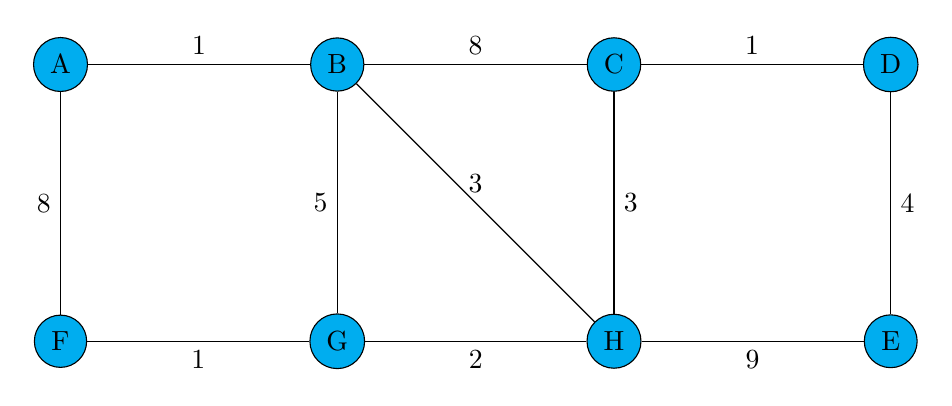
\begin{tikzpicture}
            \tikzstyle{main node}=[draw,auto,node distance=100pt,circle,align=center,fill=cyan]
            \node[main node] (A) {A};
            \node[main node] (B) [right of=A] {B};
            \node[main node] (C) [right of=B] {C};
            \node[main node] (D) [right of=C] {D};
            \node[main node] (E) [below of=D] {E};
            \node[main node] (F) [below of=A] {F};
            \node[main node] (G) [below of=B] {G};
            \node[main node] (H) [below of=C] {H};

            \draw (A) -- (B) node[draw=none,fill=none,midway,above] {1};
            \draw (A) -- (F) node[draw=none,fill=none,midway,left] {8};
            \draw (B) -- (C) node[draw=none,fill=none,midway,above] {8};
            \draw (B) -- (G) node[draw=none,fill=none,midway,left] {5};
            \draw (B) -- (H) node[draw=none,fill=none,midway,above] {3};
            \draw (C) -- (D) node[draw=none,fill=none,midway,above] {1};
            \draw (C) -- (H) node[draw=none,fill=none,midway,right] {3};
            \draw (D) -- (E) node[draw=none,fill=none,midway,right] {4};
            \draw (E) -- (H) node[draw=none,fill=none,midway,below] {9};
            \draw (F) -- (G) node[draw=none,fill=none,midway,below] {1};
            \draw (G) -- (H) node[draw=none,fill=none,midway,below] {2};
        \end{tikzpicture}
    \end{center}
    \color{blue}
    {\footnotesize
        \begin{tabular}{lll}
            \toprule
            Step & Confirmed & Tentative\\
            \hline
            1 & (A, 0, -) & \\
            2 & (A, 0, -) & (B, 1, B), (F, 8, F)\\
            3 & (A, 0, -), (B, 1, B) & (F, 8, F)\\
            4 & (A, 0, -), (B, 1, B) & (F, 8, F), (C, 9, B), (G, 6, B), (H, 4, B)\\
            5 & (A, 0, -), (B, 1, B), (H, 4, B) & (F, 8, F), (C, 9, B), (G, 6, B)\\
            6 & (A, 0, -), (B, 1, B), (H, 4, B) & (F, 8, F), (C, 7, B), (G, 6, B), (E, 13, B)\\
            7 & (A, 0, -), (B, 1, B), (H, 4, B), (G, 6, B) & (F, 8, F), (C, 7, B), (E, 13, B)\\
            8 & (A, 0, -), (B, 1, B), (H, 4, B), (G, 6, B) & (F, 7, F), (C, 7, B), (E, 13, B)\\
            9 & (A, 0, -), (B, 1, B), (H, 4, B), (G, 6, B), (C, 7, B) & (F, 7, F), (E, 13, B)\\
            10 & (A, 0, -), (B, 1, B), (H, 4, B), (G, 6, B), (C, 7, B) & (F, 7, F), (E, 13, B), (D, 8, B)\\
            11 & (A, 0, -), (B, 1, B), (H, 4, B), (G, 6, B), (C, 7, B), (F, 7, F) & (E, 13, B), (D, 8, B)\\
            12 & (A, 0, -), (B, 1, B), (H, 4, B), (G, 6, B), (C, 7, B), (F, 7, F) & (E, 13, B), (D, 8, B)\\
            13 & (A, 0, -), (B, 1, B), (H, 4, B), (G, 6, B), (C, 7, B), (F, 7, F), (D, 8, B) & (E, 13, B)\\
            14 & (A, 0, -), (B, 1, B), (H, 4, B), (G, 6, B), (C, 7, B), (F, 7, F), (D, 8, B) & (E, 12, B)\\
            15 & (A, 0, -), (B, 1, B), (H, 4, B), (G, 6, B), (C, 7, B), (F, 7, F), (D, 8, B), (E, 12, B) & \\
            \bottomrule
        \end{tabular}
    }
    \color{black}
% 10
\item\mbox{}\textbf{Distance-Vector Routing}\\
    Consider the following network configuration where the routers calculate shortest routes using the Distance Vector Routing Protocol.
    \begin{center}
        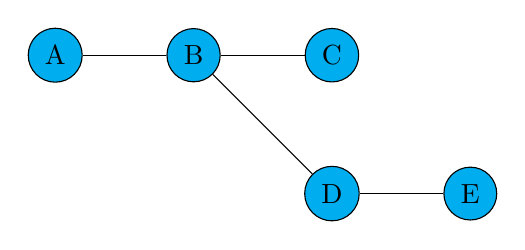
\begin{tikzpicture}
            \tikzstyle{main node}=[draw,auto,node distance=50pt,circle,align=center,fill=cyan]
            \node[main node] (A) {A};
            \node[main node] (B) [right of=A] {B};
            \node[main node] (C) [right of=B] {C};
            \node[main node] (D) [below of=C] {D};
            \node[main node] (E) [right of=D] {E};

            \draw (A) -- (B);
            \draw (B) -- (C);
            \draw (B) -- (D);
            \draw (D) -- (E);
        \end{tikzpicture}
    \end{center}
    Initially, the router tables for routes to node A look like the following:\\
    \begin{center}
        \begin{tabular}{|c|c|c|c|c|c|c|c|}
            \hline
            \multicolumn{2}{|c|}{B} & \multicolumn{2}{|c|}{C} & \multicolumn{2}{|c|}{D} & \multicolumn{2}{|c|}{E}\\
            \hline
            Cost & Next Hop & Cost & Next Hop & Cost & Next Hop & Cost & Next Hop\\
            \hline
            1 & A & 2 & B & 2 & B & 3 & D\\
            \hline
            & & & & & & & \\
            \hline
        \end{tabular}\\
    \end{center}
    Now, assume node A goes down.\\

    Given the following sequence of routing update messages, fill in the table for the routing entries for reaching A at each event, where the notation B $\rightarrow$ C indicates that node B sent a routing update to node C.\\
    \begin{center}
        \begin{tabular}{|c|c|c|c|c|c|c|c|c|}
            \hline
            & \multicolumn{2}{|c|}{B} & \multicolumn{2}{|c|}{C} & \multicolumn{2}{|c|}{D} & \multicolumn{2}{|c|}{E}\\
            \hline
            Event & Cost & Next Hop & Cost & Next Hop & Cost & Next Hop & Cost & Next Hop\\
            \hline
            & 1 & A & 2 & B & 2 & B & 3 & D\\
            \hline
            Node A goes down & & & & & & & & \\
            \hline
            C $\rightarrow$ B & & & & & & & & \\
            \hline
            B $\rightarrow$ D & & & & & & & & \\
            \hline
            D $\rightarrow$ E & & & & & & & & \\
            \hline
            E $\rightarrow$ D & & & & & & & & \\
            \hline
            D $\rightarrow$ B & & & & & & & & \\
            \hline
            B $\rightarrow$ C & & & & & & & & \\
            \hline
            C $\rightarrow$ B & & & & & & & & \\
            \hline
            B $\rightarrow$ D & & & & & & & & \\
            \hline
        \end{tabular}
    \end{center}
    Analyze this carefully and try to see what's happening compared to what should happen ideally. So what, according to you, is the problem here? Why is it a problem?\\
    \color{blue}
    \begin{tabular}{|c|c|c|c|c|c|c|c|c|}
        \hline
        & \multicolumn{2}{|c|}{B} & \multicolumn{2}{|c|}{C} & \multicolumn{2}{|c|}{D} & \multicolumn{2}{|c|}{E}\\
        \hline
        Event & Cost & Next Hop & Cost & Next Hop & Cost & Next Hop & Cost & Next Hop\\
        \hline
        & 1 & A & 2 & B & 2 & B & 3 & D\\
        \hline
        Node A goes down & $\infty$ & - & 2 & B & 2 & B & 3 & D \\
        \hline
        C $\rightarrow$ B & 3 & C & 2 & B & 2 & B & 3 & D \\
        \hline
        B $\rightarrow$ D & 3 & C & 2 & B & 4 & B & 3 & D \\
        \hline
        D $\rightarrow$ E & 3 & C & 2 & B & 4 & B & 3 & D \\
        \hline
        E $\rightarrow$ D & 3 & C & 2 & B & 4 & B & 5 & D \\
        \hline
        D $\rightarrow$ B & 3 & C & 2 & B & 4 & B & 5 & D \\
        \hline
        B $\rightarrow$ C & 3 & C & 4 & B & 4 & B & 5 & D \\
        \hline
        C $\rightarrow$ B & 5 & C & 4 & B & 4 & B & 5 & D \\
        \hline
        B $\rightarrow$ D & 5 & C & 4 & B & 6 & B & 5 & D \\
        \hline
    \end{tabular}\\
    Instead of updating routing table to ``A unreachable'', all nodes believe that A is still reachable, which is obviously contradict to the real situation. This is the well-known ``count to infinity'' problem. Nodes will keep sending updating messages and forwarding packets toward A, which is a waste of bandwidth.
    \color{black}
% 11
\item\mbox{}Explain the exposed terminal problem and how it is solved.\\
    \color{blue}
    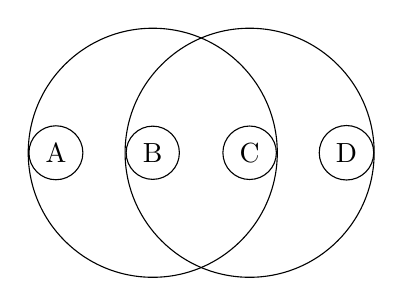
\begin{tikzpicture}
        \tikzstyle{main node}=[draw,auto,node distance=35pt,circle,align=center]
        \node[main node] (A) {A};
        \node[main node] (B) [right of=A] {B};
        \node[main node] (C) [right of=B] {C};
        \node[main node] (D) [right of=C] {D};

        \draw (B) circle (45pt);
        \draw (C) circle (45pt);
    \end{tikzpicture}\\
    B transmits to A, C hears B, C refuses to transmit to D.\\
    MACA solution: If C sees a RTS without a CTS, C can transmit.
    \color{black}
% 12
\item\mbox{}Name the OSI layer or layers in which medium access control (MAC) is addressed and state whether MAC is typically handled in hardware, in software, or in both in the Internet architecture.\\
    \color{blue}
    MAC is addressed in the data link layer, and is typically handled in hardware.
    \color{black}
% 13
\item\mbox{}Give two good reasons to allow branching - that is, the ability to support multiple protocols above and below any given protocol - in protocol graphs.
    \color{blue}
    \begin{itemize}
    \item Can use same protocol over different mediums.
    \item Can use different protocols over same network.
    \end{itemize}
    \color{black}
% 14
\item\mbox{}Explain one advantage of abstracting networked communication into multiple layers.\\
    \color{blue}
    Communication Network with multiple layers is easier to maintain. For example, if a network goes down, we can examine layer by layer instead of the entire network.
    \color{black}
% 15
\item\mbox{}Explain how a receiver detects the end of a frame with length-based framing.\\
    \color{blue}
    The receiver detects the end of a frame by looking at the length of the payload stored in the frame header.
    \color{black}
% 16
\item\mbox{}Name the OSI layer or layers in which framing is addressed and state whether framing is typically handled in hardware, in software, or in both in the internet architecture.\\
    \color{blue}
    Framing is addressed in the data link layer, and is typically handled in hardware.
    \color{black}
% 17
\item\mbox{}Explain two methods of solving the problem of communicating between machines with mixed endianness on a network.
    \color{blue}
    \begin{itemize}
    \item Let two machines to synchronize their endian first then decide which endian to use.
    \item Use a standard endian in network connection. For example, all communicate in big endian.
    \end{itemize}
    \color{black}
% 18
\item\mbox{} Explain how a receiver detects the end of a frame with sentinel-based framing.\\
    \color{blue}
    The end of the frame must be marked with a special byte or bit pattern so that the receiver can detect whether the frame ends or not.
    \color{black}
% 19
\item\mbox{}What is head-of-line blocking, and when does it occur?\\
    \color{blue}
    Head-of-line blocking coours when a line of packets is held up by the first packet. The packets in the back need to wait for the first packet even if they are not contending resources.
    \color{black}
% 20
\item\mbox{}Define the Hamming distance of an encoding.\\
    \color{blue}
    The minimum number of bit flips to move from one code to another.
    \color{black}
% 21
\item\mbox{}Explain the effect of layering on end-to-end bandwidth.\\
    \color{blue}
    The more layering generally means longer header in the data packet. Thus it will lower the end-to-end bandwidth.
    \color{black}
% 22
\item\mbox{}Name the OSI layer of layers in which encoding is addressed and state whether encoding is typically handled in hardware, in software, or in both in the Internet architecture.\\
    \color{blue}
    Encoding is addressed in the data link layer, and is typically handled in hardware.
    \color{black}
% 23
\item\mbox{}Explain a drawback of forwarding packets with source routing.
    \color{blue}
    \begin{itemize}
    \item Hosts need to know entire network topology
    \item Large headers
    \item Hosts must learn for all changes in the network
    \end{itemize}
    \color{black}
% 24
\item\mbox{}What delay is relevant and what bandwidth is relevant for computing the delay-bandwidth product of two links in series?\\
    \color{blue}
    Sum of all delays are relevant and only the smallest bandwidth is relevant because it is the bottleneck
    \color{black}
% 25
\item\mbox{}Describe a problem associated with communicating between heterogeneous architectures (e.g., a mixture of Sun and Intel hosts) on a network.\\
    \color{blue}
    The endianness may be a problem associated with communicating between heterogeneous architectures on a network.
    \color{black}
% 26
\item\mbox{}What purposes do the four addresses in an IEEE 802.11 packet serve?\\
    \color{blue}
    An 802.11 frame can have up to four address fields. Each field can carry a MAC address. Address 1 is the receiver, address 2 is the transmitter, and address 3 is used for filtering purposes by the receiver.
    \color{black}
% 27
\item\mbox{}Show that the final parity check in a horizontal and vertical parity check code, if taken as the modulo 2 sum of all data bits, is equal to the modulo 2 sum of the horizontal parity checks and also equal to the modulo 2 sum of the vertical parity checks.\\
    \color{blue}
    Example:\\
    \begin{tabular}{cccc|c}
        1 & 0 & 1 & 1 & 1\\
        0 & 1 & 1 & 0 & 0\\
        0 & 1 & 1 & 1 & 1\\
        1 & 0 & 0 & 0 & 1\\
        1 & 1 & 0 & 0 & 0\\
        1 & 0 & 0 & 1 & 0\\
        \hline
        0 & 1 & 1 & 1 & 1\\
    \end{tabular}
    modulo 2 sum of all data bits $= 1$\\
    modulo 2 sum of the horizontal parity checks $= 1$\\
    modulo 2 sum of the vertical parity checks $= 1$\\
    \color{black}
% 28
\item\mbox{} \sout{Explain how a receiver detects the end of a frame with clock-based framing (e.g., SONET).}
% 29
\item\mbox{} Explain what frequency-hopped spread spectrum modulation is, and a motivation for using it.\\
    \color{blue}
    Frequency-hopped spread spectrum modulation transmit over a random sequence of frequency, and the motivation for using it is to prevent from jamming and snooping by attackers.
    \color{black}
% 30
\item\mbox{}Suppose packets on a wireless link consist of $N$ data bits and $H$ header bits each, where $H$ is fixed. Suppose bits are received in error with probability $P$, independently of each other, and that $N$ is adjusted to maximize the throughput of data in bits per second. If $P$ gets larger, does the optimal value of $N$ get larger or smaller? Why?\\
    \color{blue}
    The probability for a packet to be received in success $= (1 - P)^{N+H}$\\
    $\Rightarrow$ throughput in bits per second $= (1 - P)^{N+H} \times N \times \frac{B}{N + H}$\\
    where $B$ is the bandwidth\\
    $\because (1 - P)^{N+H}$ is more sensitive to change of $N$\\
    $\therefore$ as $P$ gets larger, $N$ should get smaller to give the maximum throughput
    \color{black}
% 31
\item\mbox{}Name the four components that uniquely specify a TCP connection and state the length of each component in bits.
    \color{blue}
    \begin{itemize}
    \item Source address: 32 bits for IPv4
    \item Source port: 16 bits
    \item Destination address: 32 bits for IPv4
    \item Destination port: 16 bits
    \end{itemize}
    \color{black}
% 32
\item\mbox{}Consider a frame consisting of two characters of four bits each. Assume that the probability of error is $10^{-3}$, independent for each bit. What is the probability that the frame is received correctly? And a parity bit to each character. Now what is the probability?\\
    \color{blue}
    $(1 - 10^{-3})^8 \simeq 0.992 = 99.2\%$\\
    $(1 - 10^{-3})^{10} \simeq 0.990 = 99.0\%$
    \color{black}
% 33
\item\mbox{}State an advantage of direct memory access (DMA) over programmed input/output (PIO).\\
    \color{blue}
    CPU is free during data transfer.
    \color{black}
% 34
\item\mbox{}Name the OSI layer or layers in which error detection is addressed in the Internet architecture and state whether error detection is typically handled in hardware, in software, or in both.\\
    \color{blue}
    CRC check is addressed in the data link layer, and is typically handled in hardware.\\
    IP checksum is addressed in the network layer, and is typically handled in software.
    \color{black}
% 35
\item\mbox{}Name and explain two effects that complicate the process of signal transmission.
    \color{blue}
    \begin{itemize}
        \item clock recovery problem: The receiver and the sender's clocks need to be synchronize to recover the bits which are sent
    \item continuous 0s or 1s: Long strings of 0s confused with no signal, and long strings of 1s causes baseline wander
    \end{itemize}
    \color{black}
% 36
\item\mbox{} \sout{Explain the main drawback of the use of multiple logical channels for reliable transmission}
% 37
\item\mbox{}To provide more reliability than a single parity bit can give, an error detecting coding scheme uses one parity bit for checking all the odd numbered bits and a second parity bit for all the even numbered bits. What is the hamming distance of this code?\\
    \color{blue}
    2, only need to flip two odd bits or two even bits in the message to preserve correctness.
    \color{black}
% 38
\item\mbox{} What does 4B/5B encoding accomplish, besides expanding the number of bits by 25\%?\\
    \color{blue}
    4B/5B encoding will have at least two transitions for each code so that long strings of 0s or 1s will not occur in 4B/5B encoding.
    \color{black}
% 39
\item\mbox{}Describe the problem solved by error detection.\\
    \color{blue}
    Validate the correctness of the frame. Compare to error correction, error detection only overhead on messages with error.
    \color{black}
% 40
\item\mbox{}Explain the hidden terminal problem and how it is solved.\\
    \color{blue}
    Same as problem 11.
    \color{black}
% 41
\item\mbox{}Name and describe the type of multiplexing traditionally employed in data networks.\\
    \color{blue}
    Statistical multiplexing: Stations get access to channel as needed. Each station gets fixed length on transmission. Time-slot length is packet transmission time. Unused slots go idle only if no station has data to send.
    \color{black}
% 42
\item\mbox{}The data rate of a QAM system using $M$-ary symbols can be doubled by increasing $M$ and holding the bandwidth and baud rate constant. How must larger must $M$ be, and why?\\
    \color{blue}
    $\because$ eache symbol denotes $\log_2M$ bits\\
    $\therefore$ to double data rate, $M$ needs to increase to $M^2$, which results in $\log_2M^2 = 2\log_2M$ bits
    \color{black}
% 43
\item\mbox{}Draw a protocol graph for the Internet, including at least the following: ATM, Ethernet, FDDI, FTP, HTTP, IP, TCP, TFTP, and UDP.\\
    \color{blue}
    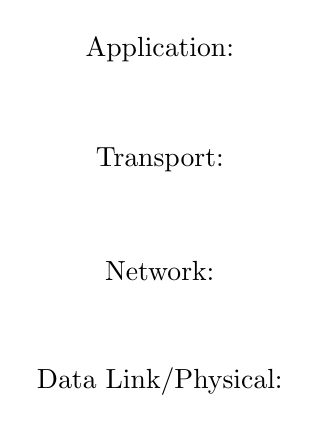
\begin{tikzpicture}
        \tikzstyle{main node}=[node distance=40pt,align=left]
        \node[main node] (Application) {Application:};
        \node[main node] (Transport) [below of=Application] {Transport:};
        \node[main node] (Network) [below of=Transport] {Network:};
        \node[main node] (Physical) [below of=Network] {Data Link/Physical:};
    \end{tikzpicture}
    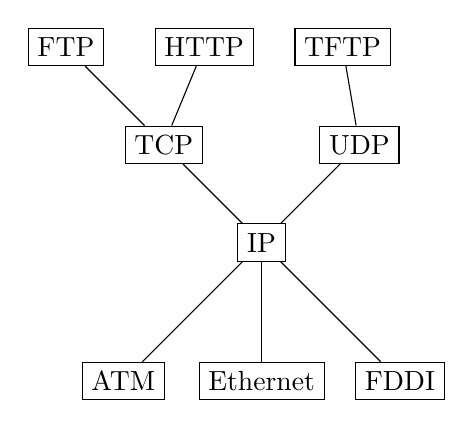
\begin{tikzpicture}
        \tikzstyle{main node}=[draw,auto,node distance=50pt,align=center]
        \node[main node] (IP) {IP};
        \node[main node] (Ethernet) [below of=IP] {Ethernet};
        \node[main node] (ATM) [left of=Ethernet] {ATM};
        \node[main node] (FDDI) [right of=Ethernet] {FDDI};
        \node[main node] (TCP) [above left of=IP] {TCP};
        \node[main node] (UDP) [above right of=IP] {UDP};
        \node[main node] (FTP) [above left of=TCP] {FTP};
        \node[main node] (HTTP) [right of=FTP] {HTTP};
        \node[main node] (TFTP) [right of=HTTP] {TFTP};

        \draw (IP) -- (ATM);
        \draw (IP) -- (Ethernet);
        \draw (IP) -- (FDDI);
        \draw (IP) -- (TCP);
        \draw (IP) -- (UDP);
        \draw (TCP) -- (FTP);
        \draw (TCP) -- (HTTP);
        \draw (UDP) -- (TFTP);
    \end{tikzpicture}
    \color{black}
% 44
\item\mbox{}In the Perlman distributed spanning tree algorithm why, does the root bridge periodically send messages even after the tree is determined?\\
    \color{blue}
    It makes sure none of the links or bridges on the tree have failed.
    \color{black}
% 45
\item\mbox{}Name the OSI layer or layers in which reliable transmission is addressed and state whether reliable transmission is typically handled in hardware, in software, or in both in the Internet architecture.\\
    \color{blue}
    Relaible transmission is addressed in the transport layer, and is typically handled in software.
    \color{black}
% 46
\item\mbox{}What Hamming distance is necessary for n-bit error detection? n-bit error correction?
    \color{blue}
    \begin{itemize}
    \item n-bit error detection:\\
        No code word changed into another code word
        $\Rightarrow$ required Hamming distance $= n + 1$
    \item n-bit error correction:\\
        No overlap between n-bit neighborhoods\\
        $\Rightarrow$ required Hamming distance $= 2n + 1$
    \end{itemize}
    \color{black}
% 47
\item\mbox{}Why are many new local area networks built using multi-mode fiber, despite the fact that single-mode fiber provides higher capacities?\\
    \color{blue}
    Single-mode fiber is powered by lasers, which requires more expensive optical-electrical interfaces.\\
    Multi-mode fiber is driven by cheap LEDs, and fits most short-range requirements.
    \color{black}
% 48
\item\mbox{} Explain a drawback of datagram-based forwarding.
    \color{blue}
    \begin{itemize}
    \item Header requires full unique address
    \item Might not be possible to deliver packet
    \item Successive packets may not follow the same route
    \item Global address to path translations requires significant storage
    \end{itemize}
    \color{black}
% 49
\item\mbox{}State the recursive definition of a network.\\
    \color{blue}
    Network is network connecting to other network.
    \color{black}
% 50
\item\mbox{}Explain a drawback of virtual-circuit-based forwarding\\
    \color{blue}
    Overhead of setting up the virtual circuit depending on the round trip.
    \color{black}
% 51
\item\mbox{}Why is byte stuffing necessary with some sentinel-based framing schemes?\\
    \color{blue}
    Because sentinel-based framing is marked with special byte or bit patterns, and these frame markers may exist in data. Therefore, it is necessary to escape such sequence.
    \color{black}
% 52
\item\mbox{}Explain why a CSMA/CD type protocol cannot be used in a wireless environment.\\
    \color{blue}
    Most radios are half-duplex, which means that they cannot listen for collision while transmitting. Therefore, collisions may not be detected by the sender.
    \color{black}
% 53
\item\mbox{}For a small data packet, which is more relevant, bandwidth or latency? Explain.\\
    \color{blue}
    Latency, because propagation delay dominates if the packet is small and transmission delay dominates if the packet is large.
    \color{black}
% 54
\item\mbox{}Explain the benefits gained by framing.\\
    \color{blue}
    A benefit gained by framing is efficient error detection. By breaking up the entire message into recoverable chunks, each chunks can be checked for error and resent instead of checking the entire message.
    \color{black}
% 55
\item\mbox{}Under what circumstances will error detection using CRC fail?\\
    \color{blue}
    Errors which is a multiple of CRC will cause the CRC error detection fail.
    \color{black}
% 56
\item\mbox{}Describe the benefits of error correction over error detection.\\
    \color{blue}
    Error correction can recover errors immediately without a retransmission.
    \color{black}
% 57
\item\mbox{}In Ethernet, how does a sender detect a collision?\\
    \color{blue}
    If a sender detects some bits transmit from other hosts, then the sender detect a collision.
    \color{black}
% 58
\item\mbox{} Why does Ethernet use binary exponential backoff during contetion resolution?\\
    \color{blue}
    Ethernet doubles maximum backoff for the next round because doing so can let the next round have less possibility to occur a collision.
    \color{black}
% 59
\item\mbox{}Describe the role of the receiver in Ethernet. How is this different from the role of the receiver in IEEE 802.11?
    \color{blue}
        \begin{itemize}
        \item Ethernet: receiver just pull the packet from the network
        \item IEEE 802.11: receiver is more active, not only pulling packets from the network, it also sends CTS and ACK to senders and other nodes
        \end{itemize}
    \color{black}
% 60
\item\mbox{}Why does Ethernet have a minimum packet size? How is it determined?\\
    \color{blue}
    Because Ethernet needs to detect collisions, and the minimum packet size must let senders still sending after $2T$, where $T$ is the propagation delay to the other host.
    \color{black}
% 61
\item\mbox{}What do ``learning'' bridges actually lean? What do the use this information for?\\
    \color{blue}
    ``Learning'' bridges learn which hosts live on which LAN. They use the information to maintain forwarding table and reduce redundant transmission.
    \color{black}
% 62
\item\mbox{}What are the limitations of bridges?\\
    \color{blue}
    Bridges are not scalable and are not heterogeneous.
    \color{black}
% 63
\item\mbox{}How do sniffers work? Will they work on all networks?\\
    \color{blue}
    Sniffers eavesdrop the packest on the shared media. Sniffers only work on networks broadcast.
    \color{black}
% 64
\item\mbox{}Why does Ethernet used fixed time slots during backoff? What could go wrong if the fixed slots were not used?\\
    \color{blue}
    Fixed time slot can make sure that all messages are sent before a host can send a message again. If the fixed time slot is not used, there might be messages in transiting and it will cause more collision when hosts try to send a message.
    \color{black}
% 65
\item\mbox{}
% 66
\item\mbox{}
% 67
\item\mbox{}
% 68
\item\mbox{} Describe ``label swapping'', and how it is used when setting up virtual circuits.\\
    \color{blue}
    Label swapping maps the VCI to a new value at each hop. Therefore, a packet just needs to follow VCI at each hop after setting up virtual circuits.
    \color{black}
% 69
\item\mbox{}
% 70
\item\mbox{}
% 71
\item\mbox{}
% 72
\item\mbox{}
% 73
\item\mbox{}
% 74
\item\mbox{}Why is determining and handling byte order left up to the programmer and not handled by the operating system?\\
    \color{blue}
    Because when data link does the ``Encoding'', data link layer does not know what byte order the system use. Programmer has to change the network byte order into system byte order.
    \color{black}
% 75
\item\mbox{}
% 76
\item\mbox{}
% 77
\item\mbox{}
% 78
\item\mbox{} Why can 4B/5B encoding be transmitted using NRZI?\\
    \color{blue}
    Because after encoding every four bits as a five bit symbol, each symbol has at least two 1s, which means that using NRZI guarantees at least two transitions for each code.
    \color{black}
% 79
\item\mbox{}
% 80
\item\mbox{}
% 81
\item\mbox{}
% 82
\item\mbox{}
% 83
\item\mbox{}
% 84
\item\mbox{}What is the impact of using different interframe spacing in IEEE 802.11?\\
    \color{blue}
    It creates different priority levels for different types of traffic.
    \color{black}
% 85
\item\mbox{}
% 86
\item\mbox{}
% 87
\item\mbox{}
% 88
\item\mbox{} In a multihop wireless network, why can't the full link bandwidth be utilized on all links?\\
    \color{blue}
    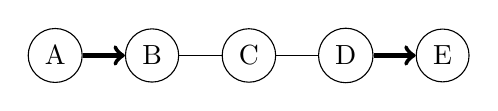
\begin{tikzpicture}
        \tikzstyle{main node}=[draw,auto,node distance=35pt,circle,align=center]
        \node[main node] (A) {A};
        \node[main node] (B) [right of=A] {B};
        \node[main node] (C) [right of=B] {C};
        \node[main node] (D) [right of=C] {D};
        \node[main node] (E) [right of=D] {E};

        \draw[ultra thick,->] (A) -- (B);
        \draw[ultra thick,->] (D) -- (E);
        \draw[thin] (B) -- (C);
        \draw[thin] (C) -- (D);
    \end{tikzpicture}\\
    As the figure shows. When A transmits to B, C needs to be idle so that C will not interfere with B, and at this moment, D can transmit to E because D will not interfere with B.
    \color{black}
% 89
\item\mbox{}
% 90
\item\mbox{}
% 91
\item\mbox{}
% 92
\item\mbox{}
% 93
\item\mbox{}
% 94
\item\mbox{}What is the effect of setting ``infinity'' to 16 in distance vector routing?\\
    \color{blue}
    Advantage: Small limit allows fast completion of ``counting to infinity''\\
    Disadvantage: Limit the size of the network
    \color{black}
% 95
\item\mbox{}Why doesn't link-state routing scale to large networks?\\
    \color{blue}
    \color{black}
% 96
\item\mbox{}
% 97
\item\mbox{}
% 98
\item\mbox{} Explain signal-to-noise ratio.\\
    \color{blue}
    Signal-to-noise ratio (SNR) is the ratio of signal power to noise power. The lower the SNR, the higher the Bit Error Rate (BER).
    \color{black}
% 99
\item\mbox{}
% 100
\item\mbox{}
% 101
\item\mbox{}\textbf{Bit- and Byte-Stuffing}\\
    Consider a data stream of 8-bit ASCII characters with values 0 to 255. Assume that the probability of a byte assuming each possible is equal (i.e., is exactly 1/256).
    \begin{enumerate}
    \item Using the bit-stuffing protocol discussed in class, what is the average number of bits that must be stuffed (inserted) per byte in the stream?\\
    \item Answer the same question posed in part (a) for a byte-stuffing protocol in which the DLE character (value 16) must be escaped by stuffing a second DLE byte.\\
    \end{enumerate}
    Now assume that the data stream contains only value in the range 32 to 255, again with a uniform probability distribution amongst the possible values.
    \begin{enumerate}
    \item Recalcuate your answer to part (a) with the new probability distribution.\\
    \item Recalcuate your answer to part (b) with the new probability distribution.\\
    \end{enumerate}

\end{enumerate}

\end{document}
